\section{Skinning}
\subsection{Was ist Skinning?}
{ %öffnende Klammer für hintergrundbild lokal
	\usebackgroundtemplate{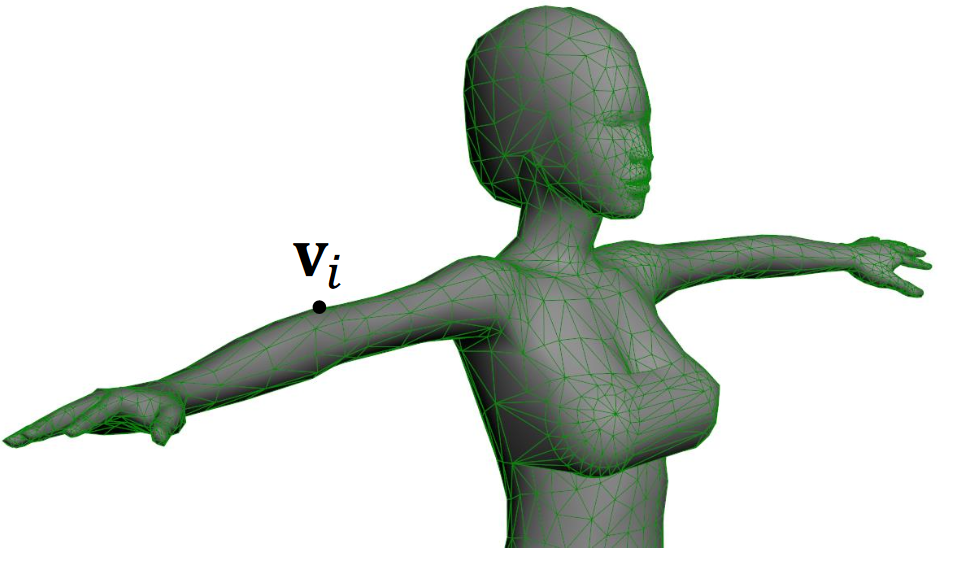
\includegraphics[width=\paperwidth,height=\paperheight]{01_Skinning/Pictures/SkinningIntro.PNG}}
	\begin{frame}{
			\begin{figure}
				\colorbox{black!10}{\Huge{Was ist Skinning?}}
			\end{figure}
		}
		\blfootnote{\colorbox{black!10}{Bildquelle: \cite{skinningcourse:2014}}}
		
		\pdfnote{Frage an alle: Was soll jetzt mit dem geriggten Modell passieren}
		\pdfnote{Frage an alle: Welcher Ansatz wäre hier der Intuitive}

		
	\end{frame}
} %schließende klammer für hintergrundbild lokal

{

	\begin{frame}{
						\begin{figure}
							\colorbox{black!10}{\Huge{Transformationen}}
						\end{figure}
			}
			
			\begin{figure}
				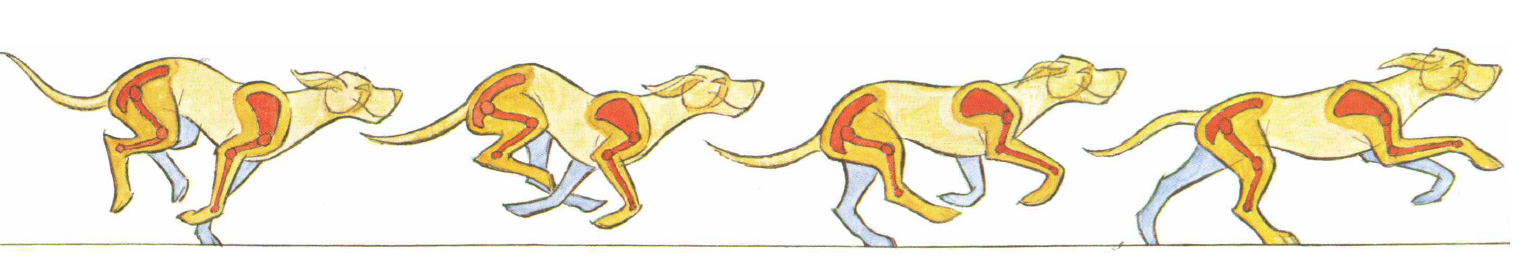
\includegraphics[width=1.0\textwidth]{01_Skinning/Pictures/Transformation.PNG}
			\end{figure}
		
		\blfootnote{\colorbox{black!10}{Bildquelle: \cite{skinningcourse:2014}}}
		
		\pdfnote{Offene Frage: Was heisst Transformation genau, wie kann man sie darstellen, was ist besonders und wichtig daran?}
		
	\end{frame}
}

{
	
	\begin{frame}{
			\begin{figure}
				\colorbox{black!10}{\Huge{Translation}}
			\end{figure}
		}
		
		\begin{figure}
			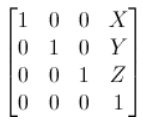
\includegraphics[width=0.3\textwidth]{01_Skinning/Pictures/Translation.PNG}
		\end{figure}
		
		
		\pdfnote{multiplikation zeigen}
		
	\end{frame}
}


{
	
	\begin{frame}{
			\begin{figure}
				\colorbox{black!10}{\Huge{Scale}}
			\end{figure}
		}
		
		\begin{figure}
			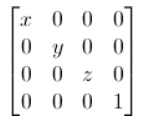
\includegraphics[width=0.3\textwidth]{01_Skinning/Pictures/scale.PNG}
		\end{figure}
		
		
		
		\pdfnote{multiplikation zeigen}
		
	\end{frame}
}

{
	
	\begin{frame}{
			\begin{figure}
				\colorbox{black!10}{\Huge{Rotation}}
			\end{figure}
		}
		
		\begin{figure}
			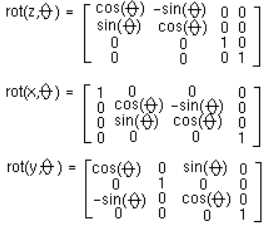
\includegraphics[width=0.6\textwidth]{01_Skinning/Pictures/rotation.PNG}
		\end{figure}
		
		
		\pdfnote{multiplikation zeigen}
		
	\end{frame}
}

{ %öffnende Klammer für hintergrundbild lokal
	\usebackgroundtemplate{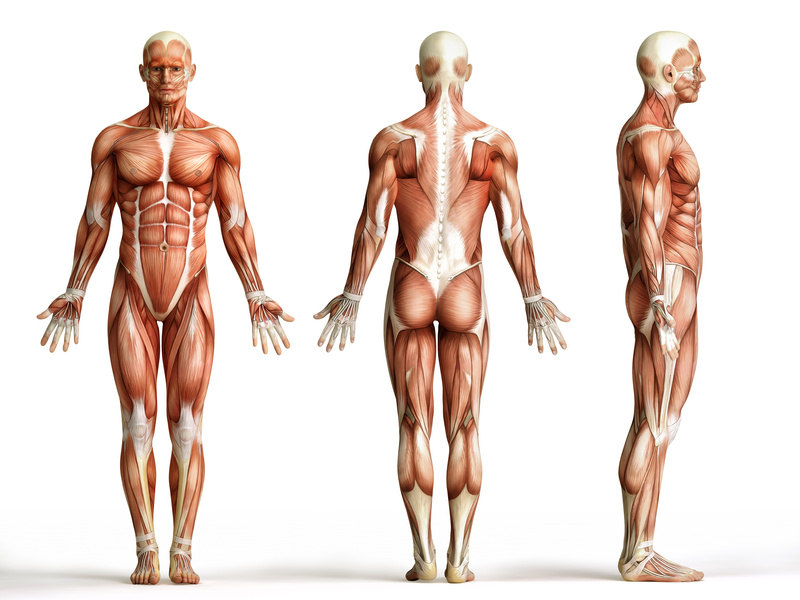
\includegraphics[width=\paperwidth,height=\paperheight]{01_Skinning/Pictures/physiologisch.jpg}}
	\begin{frame}{
			\begin{figure}
				\colorbox{black!10}{\Huge{Anatomische Modellierung}}
			\end{figure}
		}
		\blfootnote{\colorbox{black!10}{Bildquelle: \cite{muskeln}}}
		
		\pdfnote{Aufbau des Menschen abbilden -> Daraus ergibt sich Realität}
		
		
		
	\end{frame}
} %schließende klammer für hintergrundbild lokal

{
	
	\begin{frame}{
			\begin{figure}
				\colorbox{black!10}{\Huge{Motion Capture}}
			\end{figure}
		}
		
		\begin{figure}
			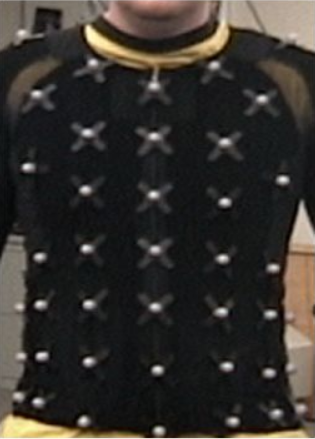
\includegraphics[width=0.6\textwidth]{01_Skinning/Pictures/breathing.PNG}
		\end{figure}
		
			\blfootnote{\colorbox{black!10}{Bildquelle: \cite{dilorenzo2008breathing}}}
		
		\pdfnote{Beobachting menschlicher Funktion}
		
	\end{frame}
}

	\begin{frame}{
			\begin{figure}
				\colorbox{black!10}{\Huge{Multipler Input}}
			\end{figure}
		}
		
		\begin{figure}
			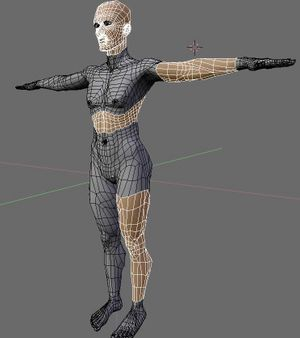
\includegraphics[width=0.6\textwidth]{01_Skinning/Pictures/multi.jpg}
		\end{figure}
		
		\blfootnote{\colorbox{black!10}{Bildquelle: \cite{multi}}}
		
		\pdfnote{Viel Input}
		
	\end{frame}


{ %öffnende Klammer für hintergrundbild lokal
	\usebackgroundtemplate{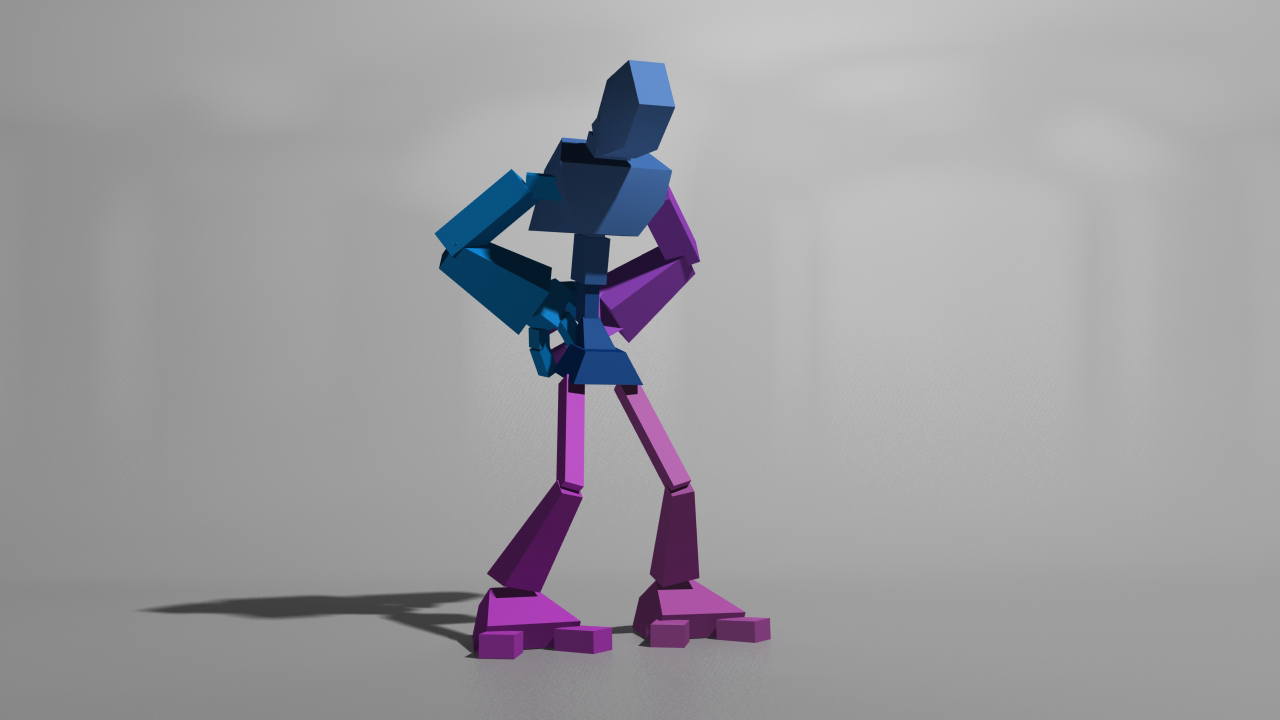
\includegraphics[width=\paperwidth,height=\paperheight]{01_Skinning/Pictures/geometrisch.jpg}}
	\begin{frame}{
			\begin{figure}
				\colorbox{black!10}{\Huge{Geometrisches Skinning}}
			\end{figure}
		}
		\blfootnote{\colorbox{black!10}{Bildquelle: \cite{geo}}}
		
		\pdfnote{Knoten an Knochen}
		
		
		
	\end{frame}
} %schließende klammer für hintergrundbild lokal
\subsection{Lineares Modell}
	\begin{frame}{
			\begin{figure}
				\colorbox{black!10}{\Huge{Linear Skinning}}
			\end{figure}
		}
		
		$$v'=Wi(v)$$
		
		\pdfnote{Lineares Modell erklären}
		
	\end{frame}

{ %öffnende Klammer für hintergrundbild lokal
	\usebackgroundtemplate{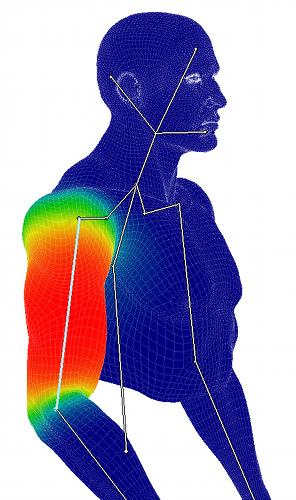
\includegraphics[width=\paperwidth,height=\paperheight]{01_Skinning/Pictures/weight.png}}
	\begin{frame}{
			\begin{figure}
				\colorbox{black!10}{\Huge{Weights}}
			\end{figure}
		}
		\blfootnote{\colorbox{black!10}{Bildquelle: \cite{weights}}}
		
		\pdfnote{Abhängigkeit vom Knochen}
		
		
		
	\end{frame}
} %schließende klammer für hintergrundbild lokal

	\begin{frame}{
			\begin{figure}
				\colorbox{black!10}{\Huge{Heat Equilibrium}}
			\end{figure}
		}
		
		\begin{figure}
			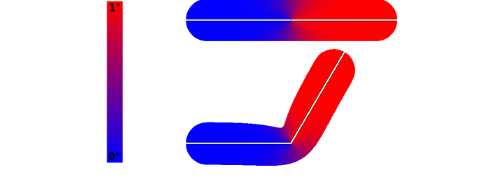
\includegraphics[width=0.6\textwidth]{01_Skinning/Pictures/heat.png}
		\end{figure}
		
		\blfootnote{\colorbox{black!10}{Bildquelle: \cite{heat}}}
		
		\pdfnote{Aufteilung anhand von Hitze}
		
	\end{frame}
	
	\begin{frame}{
			\begin{figure}
				\colorbox{black!10}{\Huge{Linear Blend Skinning}}
			\end{figure}
		}
		
		$$v'=\sum_{i=1}^{N}wiWji(v)$$
		
		\pdfnote{Lineares Blend Skinning Modell erklären}
		
	\end{frame}
	
		\begin{frame}{
				\begin{figure}
					\colorbox{black!10}{\Huge{Linear Blend Skinning Matrix}}
				\end{figure}
			}
			
			\begin{figure}
				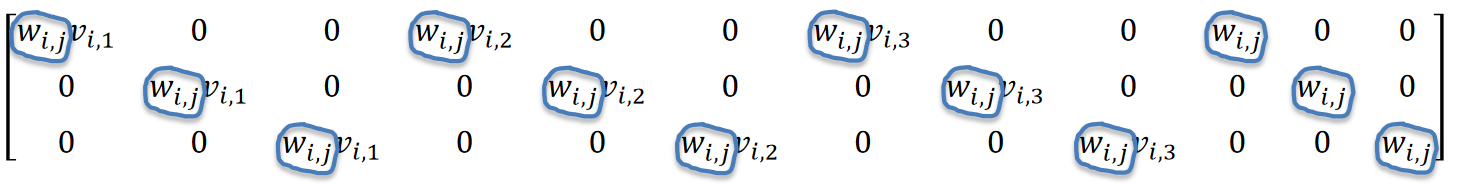
\includegraphics[width=1.0\textwidth]{01_Skinning/Pictures/lbsmatrix.png}
			\end{figure}
			
			\blfootnote{\colorbox{black!10}{Bildquelle: \cite{skinningcourse:2014}}}
			
			\pdfnote{LBS Matrix erklären}
			
		\end{frame}
		
		\begin{frame}{
				\begin{figure}
					\colorbox{black!10}{\Huge{Linear Blend Skinning Artefakte}}
				\end{figure}
			}
			
			\begin{figure}
				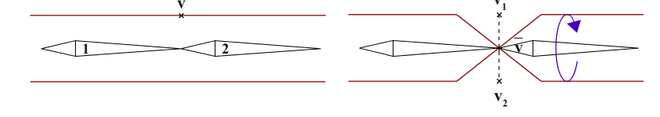
\includegraphics[width=1.2\textwidth]{01_Skinning/Pictures/rotationsartefakt.png}
			\end{figure}
			
			\blfootnote{\colorbox{black!10}{Bildquelle: \cite{weights}}}
			
			\pdfnote{Aufteilung anhand von Hitze}
			
		\end{frame}
		
				\begin{frame}{
						\begin{figure}
							\colorbox{black!10}{\Huge{Linear Blend Skinning Artefakte}}
						\end{figure}
					}
					
					\begin{figure}
						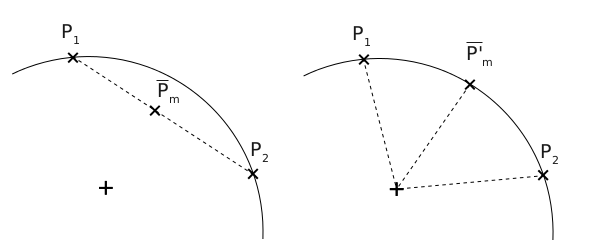
\includegraphics[width=0.6\textwidth]{01_Skinning/Pictures/interpolation_angle.png}
					\end{figure}
					
					\blfootnote{\colorbox{black!10}{Bildquelle: \cite{weights}}}
					
					\pdfnote{Aufteilung anhand von Hitze}
					
				\end{frame}

	\begin{frame}{
			\begin{figure}
				\colorbox{black!10}{\Huge{Facial Blend Skinning}}
			\end{figure}
		}
		
		$$S=S0+\sum_{i}wi(Si-S0)$$
		
		\pdfnote{Lineares Blend Skinning Modell erklären}
		
	\end{frame}

				\begin{frame}{
						\begin{figure}
							\colorbox{black!10}{\Huge{Facial Blend Skinning}}
						\end{figure}
					}
					
					\begin{figure}
						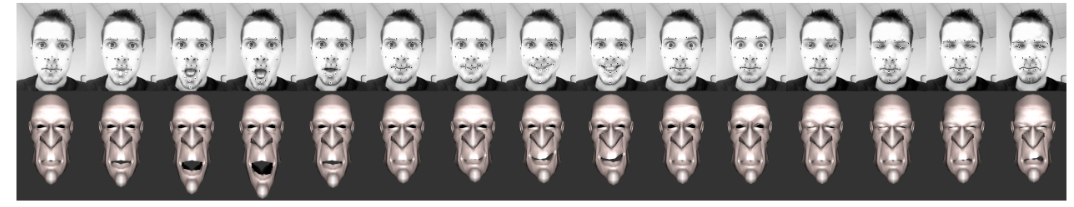
\includegraphics[width=1.2\textwidth]{01_Skinning/Pictures/face.png}
					\end{figure}
					
					\blfootnote{\colorbox{black!10}{Bildquelle: \cite{dutreve2008feature}}}
					
					\pdfnote{Aufteilung anhand von Hitze}
					
				\end{frame}
\subsection{Quaternionen}
				\begin{frame}{
						\begin{figure}
							\colorbox{black!10}{\Huge{Quaternionen}}
						\end{figure}
					}
					
					\begin{figure}
						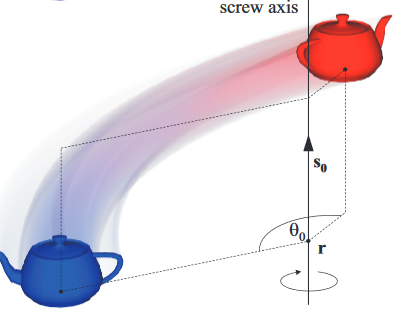
\includegraphics[width=0.5\textwidth]{01_Skinning/Pictures/Quaternionen.png}
					\end{figure}
					
					\blfootnote{\colorbox{black!10}{Bildquelle: \cite{kavan2008geometric}}}
					
					\pdfnote{Video 1}
					
				\end{frame}
				
		\begin{frame}{
				\begin{figure}
					\colorbox{black!10}{\Huge{Dual Quaternionen Skinning}}
				\end{figure}
			}
			
			$$\mathbf{\dot q} =  \frac{\sum_{i=1}^n w_i \mathbf{\dot q}_i}{\| \sum_{i=1}^n w_i \mathbf{\dot q}_i \|}$$
			
			\pdfnote{Lineares Blend Skinning Modell erklären}
			
		\end{frame}
		
				\begin{frame}{
						\begin{figure}
							\colorbox{black!10}{\Huge{Linear Blend Skinning}}
						\end{figure}
					}
					
					\begin{figure}
						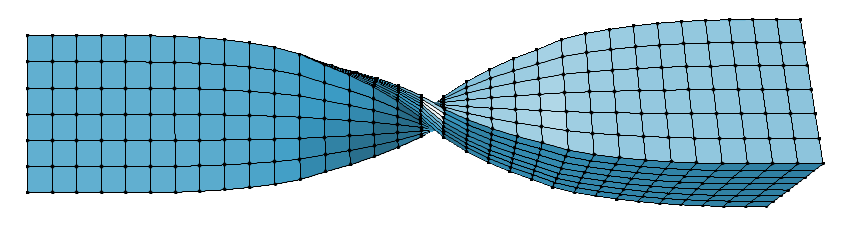
\includegraphics[width=1.0\textwidth]{01_Skinning/Pictures/lbsgrad.png}
					\end{figure}
					
					\blfootnote{\colorbox{black!10}{Bildquelle: \cite{weights}}}
					
					\pdfnote{Aufteilung anhand von Hitze}
					
				\end{frame}
				
						\begin{frame}{
								\begin{figure}
									\colorbox{black!10}{\Huge{Dual Quaternion Skinning}}
								\end{figure}
							}
							
							\begin{figure}
								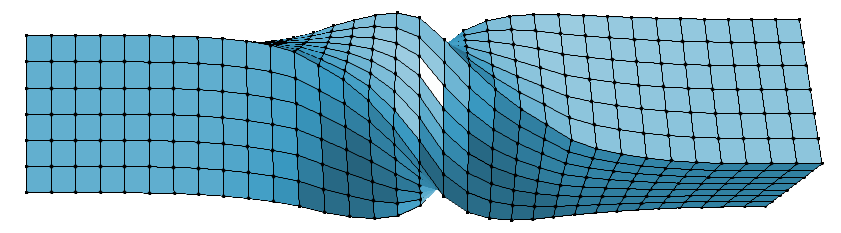
\includegraphics[width=1.0\textwidth]{01_Skinning/Pictures/dqsgrad.png}
							\end{figure}
							
							\blfootnote{\colorbox{black!10}{Bildquelle: \cite{weights}}}
							
							\pdfnote{Aufteilung anhand von Hitze}
							
						\end{frame}
						
				\begin{frame}{
						\begin{figure}
							\colorbox{black!10}{\Huge{Artefakte Dual Quaternionen}}
						\end{figure}
					}
					
					\begin{figure}
						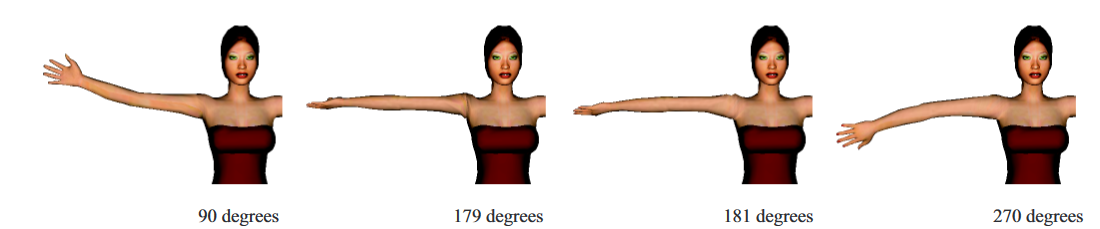
\includegraphics[width=1.0\textwidth]{01_Skinning/Pictures/dqsgradartefakte.png}
					\end{figure}
					
					\blfootnote{\colorbox{black!10}{Bildquelle: \cite{kavan2008geometric}}}
					
					\pdfnote{Video 1}
					
				\end{frame}
				
						\begin{frame}{
								\begin{figure}
									\colorbox{black!10}{\Huge{Fazit}}
								\end{figure}
							}
							
							\begin{figure}
								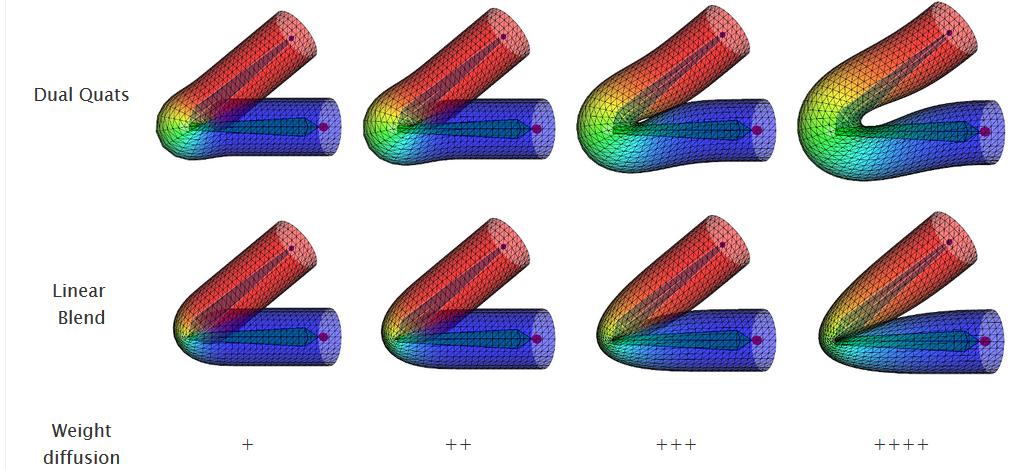
\includegraphics[width=0.8\textwidth]{01_Skinning/Pictures/lbsvsdqs.png}
							\end{figure}
							
							\blfootnote{\colorbox{black!10}{Bildquelle: \cite{weights}}}
							
							\pdfnote{Zusammenfassung, video 2}
							
						\end{frame}
		
		
	